\documentclass[reprint,aps,prb]{revtex4-1}

% Language and font encodings
\usepackage[english]{babel}

% Useful packages
\usepackage{graphicx}
\usepackage{amsmath,amsfonts,amssymb,amsthm}
\usepackage{mathtools,braket}
\usepackage{tikz}%,pgfplots}
\usepackage{xifthen}
%\pgfplotsset{compat=1.15}

% notation for standard math
\renewcommand{\d}{\partial}
\newcommand{\half}{\frac{1}{2}}
\newcommand{\dd}{{\rm d}}
\renewcommand{\r}{{\bf r}}
\newcommand{\br}{\bar{\bf r}}
\newcommand{\x}{{\bf x}}
\newcommand{\eps}{\epsilon}
\newcommand{\bomega}{\bar\omega}
\newcommand{\bbomega}{\bar{\bomega}}
\newcommand{\ii}{\mathrm{i}}
\newcommand{\intdef}[3]{\int_{#1}^{#2} \dd {#3}}
\newcommand{\intover}[1]{\int_{-\infty}^{+\infty} \dd {#1}}
\newcommand{\sint}{\mathrlap{\displaystyle\int}
\mathrlap{\textstyle\sum}
\phantom{\mathrlap{\displaystyle
\int}\textstyle\sum}}

% notatiotion for equation environments
\newcommand{\be}{\begin{equation}}
\newcommand{\ee}{\end{equation}}
\newcommand{\ba}{\begin{eqnarray}}
\newcommand{\ea}{\end{eqnarray}}
\newcommand{\baa}{\begin{align}}
\newcommand{\eaa}{\end{align}}
\newcommand{\nn}{\notag}
\newcommand{\qq}{\qquad}
\newcommand{\lb}{\label}
\newcommand{\mat}[1]{\begin{pmatrix} #1\end{pmatrix}}

% notation for the operators
\newcommand{\op}[1]{\hat {#1}}
\newcommand{\sop}[1]{\op{\op {#1}}}
\newcommand{\commutator}[2]{\left[ {#1} , {#2} \right]}
\newcommand{\trace}[1]{\mathrm{tr}\left(#1\right)}
\newcommand{\argument}[1]{\ifthenelse{\isempty{#1}{}}{}{(#1)}}
\newcommand{\matop}[1]{\mathbf{#1}}
\newcommand{\optr}[1]{\check #1}
\newcommand{\opskew}[1]{{\op {#1}}_{\perp}}

% notation for the states
\newcommand{\tket}[1]{| \tilde #1 \rangle}
\newcommand{\tbra}[1]{\langle \tilde #1 |}
\newcommand{\brket}[2]{\langle  #1 | #2 \rangle} %standard braket
\newcommand{\tbraket}[2]{\langle \tilde #1 | #2 \rangle}
\newcommand{\ketbra}[2]{| #1 \rangle \langle #2 |}
\newcommand{\tketbra}[2]{| #1 \rangle \langle \tilde #2 |}
\newcommand{\sket}[2]{| #2)^{#1}}
\newcommand{\sbra}[2]{( #2|_{#1}}
\newcommand{\sketor}[2]{| #2]^{#1}}
\newcommand{\sbraor}[2]{[ #2|_{#1}}
\newcommand{\sbraket}[2]{\braket{\op{#1} | \op{#2}}}
\newcommand{\dket}[1]{\Bigl| #1 \Bigr)}
\newcommand{\dbra}[1]{\Bigl(#1 \Bigr|}
\newcommand{\dbraket}[2]{\Bigl(#1 \Bigl| #2 \Bigr)}
\newcommand{\dketor}[1]{\Bigl| #1 \Bigr]}
\newcommand{\dbraor}[1]{\Bigl[#1 \Bigr|}
\newcommand{\hket}[1]{| #1 ]}
\newcommand{\hbra}[1]{[ #1 |}
\newcommand{\hbraket}[2]{[#1 | #2 ]}

% special operators
\newcommand{\dmnot}{\op{\rho}_0}
\newcommand{\dm}{\op{\rho}}
\newcommand{\hnot}{\op{H}_0}
\newcommand{\hone}[1]{\op{H}_1\argument{#1}}
\newcommand{\transition}[1]{\op T_{#1}}
\newcommand{\excite}[2]{\op e_{{#1}{#2}}}
\newcommand{\decay}[2]{\op d_{{#1}{#2}}}
\newcommand{\Liouv}{\sop{\mathcal L}}
\newcommand{\Liouvnot}{\sop{\mathcal L_0}}
\newcommand{\coupl}{\sop{\mathcal K}}
\newcommand{\honetmp}[1][]{\op{H_1}\argument{#1}} 
\newcommand{\identity}{\op{\mathbb I}}
\newcommand{\rmat}[1]{\optr R}


\begin{document}

%\preprint{APS/123-QED}

\title{On the analytic structure of the linear response susceptibility in open systems}
%\title{Effects of the basis set on the linear response for open systems}

\author{Luigi Genovese}
\affiliation{Laboratoire de Simulation Atomistique (LSim), SP2M, INAC, CEA-UJF, 17 Av. des Martyrs,
38054 Grenoble, France}
\author{Marco D'Alessandro}%
\affiliation{Istituto di Struttura della Materia-CNR (ISM-CNR), Via del Fosso del Cavaliere 100, 00133 Roma, Italia}

\date{\today}

\begin{abstract}
We analyze how the fundamental equations which govern the linear response properties of a quantum system are influenced by the presence of open boundaries.
In particular we focus our attention on linear-response (LR)-TDDFT calculation of molecular systems. We show that optical excitations of energy below the LR ionization potential 
behave as observable, localized quantities, that can be computationally calculated with high precision, provided an adequate level of completeness.
Above this energy threshold, the analytic structure of the susceptibility functional might be separated in two sectors: one can still be described in terms of observable excitation 
with discrete energies, that can be captured within computational setups tailored for localized states. However such excitations are embedded in a continuum of excited states 
that, on the contrary, behave as plane waves and cannot be described efficiently by the same computational techniques. Such excitations do not exhibit observable features and 
\emph{cannot} be considered as poles of the dynamical polarizability. Nonetheless, the contribution of such continuum of excitation reveals to be of paramount importance even 
for expressing LR quantities in the infrared regime like for example static polarizability.
This is particularly evident for small molecules; we show how these considerations might be influenced by the size of molecular system.
We then present indicators that can help to quantify such potential observable property of an excitation, that can be evaluated 
in any discretization scheme.  This result is a inherent behavior of the system's Liouvillian, and does not depend on computational treatment of the 
unoccupied subspace.
\end{abstract}

%\pacs{Valid PACS appear here}
\maketitle

\section{Introduction}

The subject of the present investigation concerns with the study of isolated molecular-like systems subjected to a time-dependent perturbation. % in the linear response regime.
This problem can be tackled within the contest of the time-dependent density functional theory (TD-DFT)\cite{runge1984,onida2002}, that allows one to establish the time-dependent 
Kohn-Sham (KS) equations which determine the evolution of the one-particle properties of the system with respect to time. 

We focus our attention to the linear response regime (LR) in which the theory can be conveniently expressed in the frequency domain and the time-dependent KS equation are reformulated 
as a quantum Liouville equation for the response density operator. Different computational approaches have been developed in literature\cite{baroni2008,hubener2014,brabec2015}, principally 
with the aim of producing efficient algorithms for the evaluation of the physical observables. These methods differ both for the procedure adopted to solve the Liouville equation 
(explicit diagonalization, self-consistent Sternheimer equation, Lanczos chain-like procedure, etc.) and both for the choice of the basis set employed to perform the calculations. 
Nonetheless, in all the cases one is a dealing with a finite basis set that, unavoidably, gives rise to a limited computational domain. It is then meaningful to try to understand under 
which extent the computational-induced truncation of the natural open boundaries condition could produce observable effects on the physical quantities computed in the LR. 

A preliminary understanding of this problem can be achieved thanks to the results reported in\cite{boffi2016}. The authors of this paper discuss the effects of a finite basis set on the 
occupied and virtual orbitals of a molecular system and establish a clear correspondence between the orbital localization character, and the independence of its properties (\emph{e.g.} energy) 
with respect to the basis set. It is shown that (localized) orbitals with a bound-state behavior in the long range constitute a genuine discrete set and a finite basis is 
able to provide a reliable description of these states if the sampled domain contains their natural sizes. On the contrary, unbound (delocalized) orbitals form a continuum of states in the 
true system with open boundaries. For these class of objects the presence of a finite computational domain has a deeper impact since introduces a fictitious discretization of the energy levels. 
Furthermore, the energies of the unbound orbitals are not stable with respect to a change of the size of the computational domain and approach to zero as long as it is increased.  

In this paper we aim to reach a deeper understanding of the possible effects of a finite computational basis set on the LR regime in open systems. To achieve this task we try to
reformulate the relation between localization properties and basis independence for the main actors of the LR formalism. We present a discussion based on a double level analysis. First, 
we propose a localization argument directly based on the inspection of the response density operator. Then, we move to a deeper level and investigate the properties of the susceptibility 
functional, which represents the fundamental object in the contest of the linear response. Pursuing this approach we are naturally led to investigate the localization properties of excitation 
operators, that in turn emerge as the resonant channel of the spectral decomposition of the susceptibility. In this way we establish a direct relation between the concept of basis independence 
and the analytic structure of the linear response susceptibility.

% First of all it is useful to discuss the property of the ground state under this perspective. 
% Indeed, it is well known that the stability of the ground state and the localized nature of a molecular-like system ensures that the KS description of occupied states is represented 
% by a discrete set of wave functions that approaches to zero far apart from a compact region around the system's atoms. This behavior indicates that a (finite) basis set will provide 
% a reliable description of the ground state properties if it is able to sample a computational domain which contains the natural sizes of the occupied orbitals\cite{boffi2016}.
% The same arguments cannot be rigidly extended to the case in which an external time-dependent field starts acting on the system. Indeed, the perturbation drives the system out 
% from the equilibrium and the electrons sample a wider region of the state space, that will contains orbitals of both negative (bound) and positive (unbound) energies. 

\section{Theory}

We start by reviewing review the fundamental equations that govern the properties of an open quantum system in the linear response regime. We assume that our calculations are carried 
out within a highly complete real-space basis set that provides a precise description of the system in a finite computational domain. The purpose of the analysis is to determine the 
asymptotic behavior of the main building blocks of the LR in the long range. Then we discuss the relation between localization properties and dependence of the results of LR from the 
specific choice of the basis set and, in particular, from the dimension of the computation  domain. 

Linear response can be effectively applied to the analysis of the electronic excitations in molecular systems. In this framework one consider a system described by the Hamiltonian 
$\hnot$ and assume that the ground-state density $\dmnot$ has been provided. The linear response formalism allows us to evaluate the modification of the expectation value of a generic 
observable induced by a time-dependent perturbing field acting on the system. This quantity, written in the frequency domain, can be expressed through the evaluation of the 
\emph{linear response functional}
\be\lb{LinearResponseFunctDef1}
\braket{\delta\op O}(\omega) = \trace{\dm'(\omega)\op O} \;.
\ee
% where $\op O$ represents the observable\footnote{For a sake of concreteness, we are limiting our considerations to observables that do not explicitly depend on time} 
% under inspection. The modification of the ground-state density induced by the perturbation is expressed by the \emph{response density operator} $\dm'(\omega)$ that, in the linear 
% response regime, is a linear function of the perturbing field $\op\Phi(\omega)$. For this reason it is possible to define the \emph{susceptibility} superoperator, as follows:
% \be\lb{SusceptibilityDef1}
% \dm'(\omega) = \sop{{\cal R}}(\omega) \op\Phi(\omega) \;. 
% \ee
% Susceptibility describes an intrinsic feature of the unperturbed system and determines its response to \emph{any} perturbations, in the linear response regime.
Here $\op O$ represents the observable\footnote{For a sake of concreteness, we are limiting our considerations to observables that do not explicitly depend on time} under inspection 
while the \emph{response density operator} $\dm'(\omega)$ describes the modification of the ground-state density induced by the perturbation. In the contest of the linear response 
the response satisfies an equation of motion written in the form of a quantum Liouville operator (for example see \cite{baroni2008}),
\be\lb{LiouvillianRhopomegaDef1}
\left(\omega - \Liouv\right) \dm'(\omega) =  \commutator{\op\Phi(\omega)}{\dmnot} \;,
\ee
and $\op\Phi(\omega)$ represents the perturbing field acting on the system. 

\subsection{Fluctuation states. A localization argument for the response density}

The response density operator is expressed as the first-order variation of ground state density $\sum_{\{p\}} \ket{\psi_p} \bra{\psi_p}$, where the set $\{\ket{\psi_p}\}$ denote the 
occupied states, \emph{i.e} the subset of the bound eigenstates of $\hnot$ with energy $\eps_p$ lower than the Fermi level. Using this notation we denote the energy of the HOMO level 
as $\eps_h$ and identify the value of the first ionization potential with $|\eps_h|$. In what follows we will assume that the set of states $\{\ket{\psi_p}\}$ are described by real 
functions, when projected in the $\r$-representation.  

% By considering the linear order time evolution of the eigenstates of $\hnot$ in presence of the perturbation we can derive the equation of motion of the response density in the form of 
% a quantum Liouville equation (for example see \cite{baroni2008}). This procedure suggests us to introduce an explicit representation of the response density in terms of a set of 
% $\omega$-dependent \emph{fluctuation states} $\{\ket{f_p(\omega)}\}$, as follows: 
% \be\lb{rhoPrimeFluctuationStateDef1}
% \dm'(\omega) = \sum_p\left(\ketbra{\psi_p}{f_p(-\omega)} + \ketbra{f_p(\omega)}{\psi_p}\right) \;.
% \ee
% Fluctuation states are, by construction, orthogonal to the occupied eigenstates of $\hnot$. An analysis of the Liouville equation for the response density written in this fashion evidences 
% that their equations of motion are written in the form of a modified Sternheimer equation \cite{mahan1980}:
% \be\lb{fluctuationStateEqMotion1}
% \left[\omega - (\hnot-\eps_p)\right]\ket{f_p(\omega)} = \op Q_0(\op\Phi(\omega)+\op V'(\omega))\ket{\psi_p} \;,
% \ee
% where $\op Q_0=\identity-\dmnot$ is the projector in the subspace orthogonal to the occupied states of $\hnot$ and the operator $\op V'(\omega)$ is a perturbing term due to the 
% density-dependence of the unperturbed Hamiltonian.

The inspection of the linear order time evolution of the eigenstates of $\hnot$ evidence that the response density acts as a transitions operator, linking the occupied and empty subspaces 
of $\hnot$, and satisfies the \emph{transverse} condition  
\be\lb{RhopTransverseDef1}
\dm' = \dm_{\perp} \doteq \dmnot\dm'\op Q_0 + \op Q_0\dm'\dmnot
\ee
where $\op Q_0=\identity-\dmnot$ is the projector in the subspace orthogonal to the occupied states of $\hnot$. Due to this fact it is possible to introduce an explicit representation of the 
response density as follows 
\be\lb{rhoPrimeFluctuationStateDef1}
\dm'(\omega) = \sum_p\left(\ketbra{\psi_p}{f_p(-\omega)} + \ketbra{f_p(\omega)}{\psi_p}\right) \;,
\ee
where we have defined the set of $\omega$-dependent \emph{fluctuation states} $\{\ket{f_p(\omega)}\}$, that span the empty subspace of $\hnot$. 
An analysis of the Liouville equation \eqref{LiouvillianRhopomegaDef1} for the response density written in this fashion evidences that the equations of motion of fluctuation states are 
written as a modified Sternheimer equations \cite{mahan1980}
\be\lb{fluctuationStateEqMotion1}
\left[\omega - (\hnot-\eps_p)\right]\ket{f_p(\omega)} = \op Q_0(\op\Phi(\omega)+\op V'[\dm'])\ket{\psi_p} \;,
\ee
and we observe that the first-order Hamiltonian contains, apart from the perturbing field, a further term $\op V'[\dm']$ due to the density-dependence of $\hnot$.

The interesting aspect of these equations in the perspective of the present analysis is that they allow us to present a localization argument for the fluctuation 
states. To clarify this statement we split the unperturbed Hamiltonian as the sum of the kinetic $\op T$ and potential $\op V$ term and solve \eqref{fluctuationStateEqMotion1} in the form 
of a self-consistent inhomogeneous Helmholtz equation by writing:
\be\lb{rhoPrimeFluctuationStateDef2}
\ket{f_p(\omega)} = \op G_H(\omega+\epsilon_p)\ket{s(\omega)} \;,
\ee
where we have introduced the Green function of the Helmholtz operator $\op G_H(\omega) = (\omega-\op T)^{-1}$,
and the \emph{source term} is given by:
\be
\ket{s(\omega)} =  \op V\ket{f_p(\omega)} + \op Q_0(\op V'(\omega) + \op \Phi(\omega))\ket{\psi_p} \;.\nn
\ee
For open boundary conditions in three dimensions, the kernel of $\op G_H(\omega)$ in the coordinate representation reads: 
\be\lb{HelmholtzKernelDef1}
\bra{\r} \op G_H(\omega) \ket{\r'} = \frac{1}{4\pi} \begin{cases}
\frac{e^{-\alpha|\r - \r' |}}{|\r- \r' |} \;,\; & {\textrm for}\; \omega  < 0\; \\ 
\frac{e^{\ii \alpha |\r-\r' |}}{|\r-\r' |} \;, & {\textrm for} \; \omega \geq 0
\end{cases} \;,
\ee
where $\alpha = \sqrt{2|\omega|}$. 

The localization character of fluctuation states can be determined by looking at the long range behavior of \eqref{rhoPrimeFluctuationStateDef2}, projected in the $\r$-representation.
An inspection of the structure of \eqref{HelmholtzKernelDef1} evidences that, for each value of $p$, there exist a threshold value $\omega = |\eps_p|$, which govern the localization 
properties of the corresponding fluctuation state. Indeed, for $\omega > |\eps_p|$,  $\op G_H(\omega)$ behaves as a spherical wave and its convolution with the source term  gives 
raise to a $f_p(\omega,\r)$ delocalized in the whole accessible space. On the contrary, for values of $\omega < |\eps_p|$, % below the threshold,
the kernel contains an exponential damping factor and $f_p(\omega,\r)$ exhibit a bound-state behavior in the long range.   

% \vspace{0.3cm}
% \noindent{TODO: Add comment to support the localization below threshold}. Two possible way. First way, use the fact that the $\ket{f_p(0)}$ is the nothing but the $p$-\emph{th} 
% eigenstate of the perturbed Hamiltonian with perturbing field $\op\Phi(0)$. The localization of $\ket{f_p(0)}$ can be explicitly checked by solving the ground-state problem for
% this Hamiltonian. How to extended to finite values of $\omega$ below threshold? Second way. Try and iterative solution of the self-consistent Helmholtz equation (below threshold) 
% starting from a localized guess for the fluctuation state. Then state something about the the fact that is reasonable to believe that (for a proper choice of the perturbing field)
% the operators appearing in the source term keep its support compact. If we are able to state this in a appropriate way the localization argument below threshold hold. In my opinion
% this way is better.
% \vspace{0.3cm}

The localization properties of fluctuation states allows us to assess the reliability of the linear response functional computed using the given basis set. Indeed, writing the response 
density in terms of fluctuation states implies that 
\be\lb{LinearResponseFunctDef2}
\braket{\delta\op O}(\omega) = 2\sum_p \bra{\psi_p}\op O\ket{f_p(\omega)} \;,
\ee
so the computation of the linear response functional passes through the evaluation of the scalar products indicated in \eqref{LinearResponseFunctDef2}. 
We observe that there exists two distinct regimes, on the basis of value of $\omega$. The first one, which we will refer to as the \emph{below threshold regime}, is realized when $\omega$ 
is lower than the ionization potential $|\eps_h|$. In this case all the fluctuation states are below their threshold level and equation \eqref{LinearResponseFunctDef2} is expressed in terms 
of genuinely localized quantities\footnote{This consideration holds for the class of observables for which $\bra{\psi_p}\op O$ is a localized state  with bound-state behavior in the long 
range}, each of which possesses a physical cut-off radius.
Due to this behavior we can affirm that given basis provides a reliable evaluation of \eqref{LinearResponseFunctDef2} if the chosen computational domain is suitable to express the
bound-state like fluctuation states, in a analogous fashion of a ground state calculation. 

On the contrary, the computation of the linear response functional can be much more demanding in the \emph{above threshold regime}, realized for $\omega>|\eps_h|$, in which fluctuation 
states start behaving as unbound wave functions. In this case a computational description of fluctuation states is only meaningful in weak sense, \emph{i.e} inside the scalar products of 
\eqref{LinearResponseFunctDef2}, where the bound state character of $\{\bra{\psi_p}\op O\}$ behave as a regulator. This observation indicates that, above threshold, a computational setup 
provides a reliable assessment of \eqref{LinearResponseFunctDef2} only if it is able to express an unbiased description of the fluctuation states in the support of $\{\bra{\psi_p}\op O\}$. 

As an explicit example in support of these arguments we compare the absorption spectrum of a $CO$ molecule computed in three distinct real-space basis set, which differs for the dimension of 
the computational domain. Results reported in figure \ref{co_spectrum} evidences that the curves are almost coincident in the below threshold regime, whereas the effect of the computational 
setup are clearly visible in the for values of $\omega$ that exceed the threshold value. 

% This fact implies that a computational setup has different chances of providing a reliable assessment of the linear response functional \eqref{LinearResponseFunctDef2} depending
% to the value of $\omega$. 
% This observation has relevant consequence on the capability of a computational setup to provide a reliable assessment of the linear response functional....  

\begin{figure}
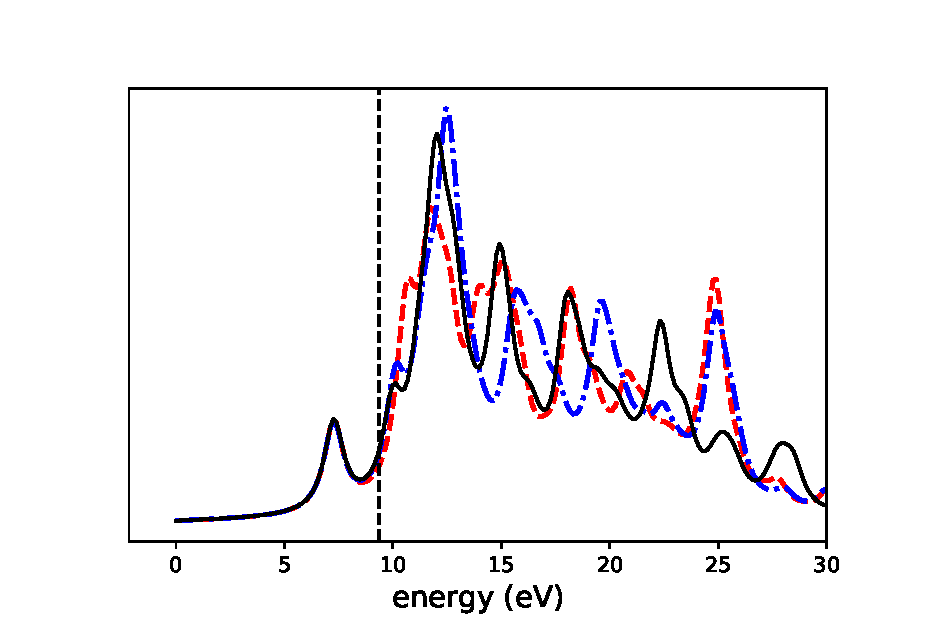
\includegraphics[scale=0.56]{co_spectrum.eps}
\caption{\label{co_spectrum}(Color online) Convergence below threshold of the $CO$ spectrum computed in different computational setup.}
\end{figure}

%This analysis, carried out starting from the representation of the linear response functional in terms of fluctuation states, evidences some general properties of the linear response. 
%In the next sections we will reformulate an analogous procedure directly looking at the susceptibility. This analysis lead us to the core of the paper, namely the description of the
%analytical structure of the linear response susceptibility. 

\subsection{Excitation operators. The analytic structure of the susceptibility functional} %Spectral decomposition of the susceptibility functional}

The localization properties of the response density can be reformulated in terms of the \emph{susceptibility functional}, implicitly defined trough the operator equation  
\be\lb{SusceptibilityDef1}
\dm'(\omega) = \sop{{\cal R}}(\omega) \op\Phi(\omega) \;. 
\ee
The main advantage of this approach relies on the fact that the susceptibility describes an intrinsic feature of the unperturbed system and its knowledge determines the LR properties 
independently from the specific choice of the perturbing field.

The analysis is based on the spectral decomposition of the Liouville equation \eqref{LiouvillianRhopomegaDef1} and the make usage of the \emph{excitation operators}, defined through the 
operator eigenvalue equation
\be\lb{ExcitationOperatorsDef1}
\Liouv \op E = E \op E \;, %\qq \op{\tilde E} \Liouv = E \op{\tilde E}
\ee
with the normalization condition $\trace{\op E\op E'} = \delta(E-E')$.
%\be
%\trace{\op E\op E'} = \delta(E-E') \;. \nn
%\ee
The properties of the Liouvillian superoperator (see appendix?) imply that excitations are transverse operators so that $\op E = \dmnot\op E\op Q_0 + \op Q_0\op E\dmnot$. 
This condition allows us to introduce a dyadic representation of excitations as follows
\be\lb{ExcitationOperatorsDef2}
\op E = \sum_p \left( \ket{\phi^E_p}\bra{\psi_p} + \ket{\psi_p} \bra{\chi^E_p}\right)\;, 
\ee
where the \emph{excited states} $\ket{\phi^E_p}$ and $\bra{\chi^E_p}$ span the domain of $\op Q_0$, \emph{i.e} the empty subspace of $\hnot$. The eigenvalue condition \eqref{ExcitationOperatorsDef1} 
can thus be recasted in the form of a Sternheimer-like equations for the excited states
\begin{align}
\left(\hnot - \eps_p\right) \ket{\phi_p^E} + \op Q_0 \op V'[\op E] \ket{\psi_p} &= E \ket{\phi_p^E} \;, \\
\bra{\chi_p^E}\left(\hnot - \eps_p\right) + \bra{\psi_p}\op V'[\op E]\op Q_0   &= -\bra{\chi_p^E} E  \;, \nn
\end{align}
and the orthonormalization condition of the excitation operators is expressed as 
\be
\sum_p \left(\braket{\phi_p^E | \phi_p^{E'}} + \braket{\chi_p^E | \chi_p^{E'}}\right) = \delta(E-E') \;. \nn
\ee



\vspace{1cm}

% Now we reformulate an analogous analysis looking at the susceptibility superoperator, implicit defined through \eqref{SusceptibilityDef1}. This approach leads to the concept of \emph{excitation 
% operators}, defined through a self-consistent operator eigenvalue equation. Excitations behave as singularity of the susceptibility operator and their knowledge provides a deeper insight 
% into the analytic structure of the linear response. 

Using the spectral decomposition of the resolvent of the Liouvillian we have:
\be\lb{RhopExcitationDef1}
\sop{{\cal R}}(\omega) \cdot   =
\left(\sum_E + \int\dd E   \right) \op E
\frac{\trace{\opskew{\tilde E}\cdot}}{\omega-E} \;,
\ee
with $\opskew{O} = \commutator{\op O}{\dmnot}$. 

\begin{figure}
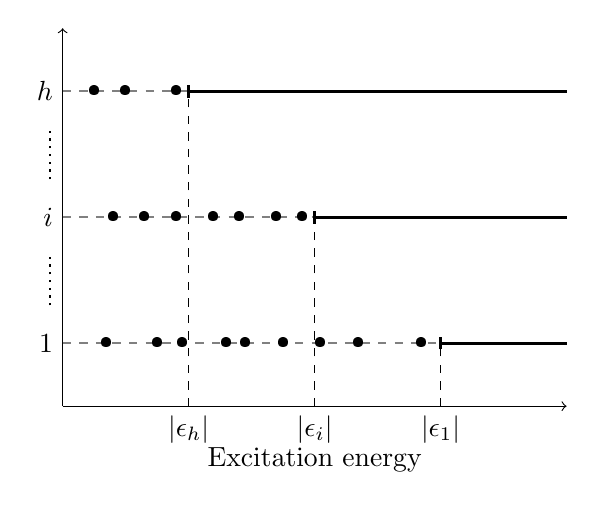
\begin{tikzpicture}[scale=0.8]
% axes
\draw[->] (0,0) -- (8,0); %node[below] {$x$};
\draw[->] (0,0) -- (0,6); %node[left] {$y$};
% orizontal lines
\draw[dashed,thick,color=gray] (0,5) -- (2,5);
\draw[very thick](2,5) -- (8,5);
\draw[dashed,thick,color=gray] (0,3) -- (4,3);
\draw[very thick] (4,3) -- (8,3);
\draw[dashed,thick,color=gray] (0,1) -- (6,1);
\draw[very thick] (6,1) -- (8,1);
% vertical lines
\draw[dashed,very thin,color=black] (2,0) -- (2,5);
\draw[dashed,very thin,color=black] (4,0) -- (4,3);
\draw[dashed,very thin,color=black] (6,0) -- (6,1);
% threshold levels labels
\node[left] at (0,5) {$h$};
\node[left] at (0,3) {$i$};
\node[left] at (0,1) {$1$};
\node[below] at (2,0){$|\eps_h|$};
\node[below] at (4,0){$|\eps_i|$};
\node[below] at (6,0){$|\eps_1|$};
\node[below] at (4,-0.5) {Excitation energy};
% bars at thresholds
%\foreach \Point in {(2,5),(4,3),(6,1)}{
%   \node at \Point {{\textbar}};%$\times$};
%}
\draw [very thick] (2,4.9) -- (2,5.1);
\draw [very thick] (4,2.9) -- (4,3.1);
\draw [very thick] (6,0.9) -- (6,1.1);

% dotted vertical lines
\draw[dotted,thick,color=black] (-0.2,3.6) -- (-0.2,4.4);
\draw[dotted,thick,color=black] (-0.2,1.6) -- (-0.2,2.4);

% discrete excitations
\foreach \Point in {(0.5,5),(1.0,5),(1.8,5),(0.8,3),(1.3,3),(1.8,3),(2.4,3),(2.8,3),(3.4,3),(3.8,3),(0.7,1),(1.5,1),(1.9,1),(2.6,1),(2.9,1),(3.5,1),(4.1,1),(4.7,1),(5.7,1)}{
    \node at \Point {\textbullet};
}




\end{tikzpicture}
\caption{\label{ExcitationLandscape} Excitation landscape.}
\end{figure}


%\subsection{Comments. The analytic structure of the linear response susceptibility}
%
%...........

\section{Applications}

...........

\section{Comments and conclusions}

The analysis carried out starting from the representation of the linear response functional in terms of fluctuation states has evidenced some general properties of the linear response
for open systems. In particular, by analyzing the asymptotic behavior of fluctuation states in long range limit, we have showed that they exhibit a bound-state character in the regime  
$\omega<|\eps_h|$. Consequently we have argued that the linear response functional, in the same $\omega$ range, provides a setup-independent result with a modest computational effort... 

%%%%%%%%%%%%%%%%%%%%%%%%%%%%%%%%%%%%%%%%%%%%%%%%%%%%%%%%%%%%%%%%%%%%%%%%%%%%%%%%%%%%%%%%%%%%%%%%%

% In the framework of the linear response formalism one is typically interested in computing the \emph{linear response functional}:
% \be\lb{LinearResponseFunctDef1}
% {\cal R}_{\op O}(\omega) = \trace{\dm'(\omega)\op O} \;,
% \ee
% that represents the perturbation-induced modification of the expectation value of an observable $\op O$\footnote{For a sake of concreteness, we are limiting our considerations 
% to observables that do not explicitly depend on time}. Here $\dm'(\omega)$ is the \emph{response density operator} that describes the $\omega$-dependent modification of the density 
% operator induced by the perturbation.
% 
% \subsection{Basic equations for the linear response formalism for electronic excitations}
% 
% The linear response formalism can be effectively applied to the analysis of the electronic excitations of molecular and condensed-matter systems, described by the (density-dependent) 
% ground-state hermitian Hamiltonian $\hnot$, coupled to an external perturbation described by the perturbing field $\op\Phi(\omega)$. The $\omega$ structure of $\op\Phi(\omega)$ codifies both 
% the intrinsic time dependence of the perturbation and the switching-on procedure, \emph{e.g.} adiabatic or sudden limit protocols. 
% 
% The response density is expressed as the first-order variation of ground state density
% \be\label{rhodef1}
% \dmnot = \sum_{\{p\}} \ket{\psi_p} \bra{\psi_p}  \;,
% \ee
% where $\{\psi_p\}$ denote the occupied states, \emph{i.e} the subset of the bound eigenstates of $\hnot$ with energy lower than the Fermi level.
% By considering the linear order time evolution of these states in presence of the perturbation we can express the response density in the $\omega$ domain as follows:
% \be\lb{rhoPrimeOmegaDef1}
% \dm'(\omega) = \ii \commutator{\dmnot}{\op A(\omega)} \;,
% \ee
% where $\op A(\omega)$ is a sum of two terms, both written as a triple convolution with the retarded/advanced Green functions $\op G_0^{\pm}$ of the unperturbed Hamiltonian:
% \be
% \op A(\omega) = \frac{1}{2\pi} \int_{-\infty}^\infty  \dd \omega'
% \op G_0^+(\omega') \left(\op \Phi(\omega)+\op V'(\omega)\right) \op G_0^-(\omega'-\omega)\;. \nn
% \ee
% The presence of the second addend is due to the density dependence of the unperturbed Hamiltonian and describes the perturbation induced by the variation of $\hnot$ under the
% action of the perturbing field. In the linear response regime this quantity can be expressed as the functional derivatives of $\hnot$ with respect to the density kernel 
% (evaluated at $\dm=\dmnot$) times the value of the induced density modification, that is:
% \be\label{VpDef1}
% \op V'(\omega)= 
% \int \dd \r \dd \r' \frac{\delta\hnot}{\delta \rho_0(\r,\r')}
% \trace{\dm'(\omega) \ket{\r} \bra{\r'}} \;.
% \ee
% 
% \subsection{Fluctuation states. A localization argument for the linear response functional}
% 
% We start this analysis by deriving an ulterior expression of the response density operator in the frequency space. We consider equation \eqref{rhoPrimeOmegaDef1} and observe that, for any 
% operator $\op O$, we may write:  
% \be
% \commutator{\dmnot}{\op O} = \dmnot \op O \op Q_0 - \op Q_0 \op O \dmnot\;,
% \ee
% where $\op Q_0= \identity - \dmnot$ is the projection operator in the subspace orthogonal to $\dmnot$. So, thanks to this relation we have that:
% \be
% \dm'(\omega) = \ii\sum_p\left(\ketbra{\psi_p}{\psi_p}\op A(\omega)\op Q_0 - \op Q_0\op A(\omega)\ketbra{\psi_p}{\psi_p}\right) \;.
% \ee
% This equation suggests us to define the \emph{fluctuation states}:
% \be\lb{fluctuationStateDef1}
% \ket{f_p(\omega)} \doteq -\ii\op Q_0\op A(\omega)\ket{\psi_p} \;, \quad
% \bra{f_p(\omega)} \doteq \bra{\psi_p}\ii\op A(-\omega)\op Q_0 \;,
% \ee
% where the $\omega$ dependence of the bra is consistent with hermitian conjugation property of the Fourier transform of a hermitian operator. Fluctuation states are, by 
% definition, orthogonal to the occupied eigenstates of $\hnot$, so that:
% \be
% \brket{f_p(\omega)}{\psi_q} = \brket{\psi_q}{f_p(\omega)} = 0 \;, \forall \, p,q,\omega \;.
% \ee
% The response density written in terms of the fluctuation states reads:
% \be\lb{rhoPrimeFluctuationStateDef1}
% \dm'(\omega) = \sum_p\left(\ketbra{\psi_p}{f_p(-\omega)} + \ketbra{f_p(\omega)}{\psi_p}\right) \;,
% \ee
% and consequently the linear response functional can be expressed as:
% \be\lb{LinearResponseFunctDef2}
% {\cal R}_{\op O}(\omega) = 
% \sum_p\left(\bra{f_p(-\omega)}\op O\ket{\psi_p} + \bra{\psi_p}\op O\ket{f_p(\omega)}\right) \;.
% \ee


%%%%%%%%%%%%%%%%%%%%%%%%%%%%%%%%%%%%%%%%%%%%%%%%%%%%%%%%%%%%%%%%%%%%%%%%%%%%%%%%%%%%%%%%%%%%%%%%%%





\bibliography{Analytic_biblio}

\end{document}
